\documentclass[xcolor={usenames,dvipsnames,svgnames}, compress]{beamer}

\usepackage{booktabs}
\usepackage{dcolumn}
\usepackage{colortbl}
\usepackage{xcolor}
\usepackage{hyperref}
\usepackage{amsmath}
\usepackage{wrapfig}
\usepackage{pifont}
\usepackage[style=authoryear-comp]{biblatex}

\usepackage[font=scriptsize]{caption}

% 
% custom colors
\definecolor{untractable_red}{RGB}{209, 25, 25}
\definecolor{tractable_green}{RGB}{0, 153, 51}

\usetheme{enziteto}

\setbeamertemplate{headline}{}

% 
% custom colors
\definecolor{untractable_red}{RGB}{209, 25, 25}
\definecolor{tractable_green}{RGB}{0, 153, 51}

\newcommand{\cmark}{\ding{51}}%
\newcommand{\xmark}{\ding{55}}

\addbibresource{../referomnia/referomnia.bib}

\begin{document}

\newlength{\custombulletheight}
\setlength{\custombulletheight}{\dimexpr0.5\ht1-0.5\ht2}

\title{Towards Representation Learning\par with Tractable Probabilistic Models}
\author{Antonio  Vergari, Nicola {Di Mauro} and Floriana Esposito}
\institute{Lacam$@$DIB$@$Uniba}
\institute{Università degli Studi di Bari}
\department{Dipartimento di Informatica}
\laboratory{LACAM Laboratory}
\group{Machine Learning}
\institutelogo{
\includegraphics[width=25pt]{figures/unibaba}}
\lablogo{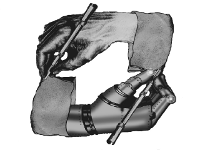
\includegraphics[width=35pt]{figures/lacam}}
\date{19th September - \textbf{ECML-PKDD} - Riva del Garda, Italy}


{
  \setbeamertemplate{headline}{}
  \setbeamertemplate{footline}{}
  \begin{frame}
    \titlepage
  \end{frame}
}

\begin{frame}[t]
  \frametitle{Tractable Probabilistic Models (TPMs)}
  \small
  Plenty of Probabilistic Models learned as \emph{density estimators}\\[6pt]
  
  Many Machine Learning problems can be reframed as probabilitic
  inference\\[6pt]
   
   \dots but \emph{\textbf{inference is hard}}.
   \begin{center}
    \begin{minipage}[t]{0.29\linewidth}
      \begin{center}
        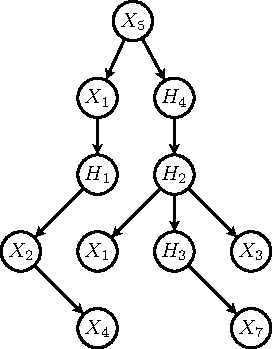
\includegraphics[width=0.8\linewidth]{figures/tree}\\
        % \begin{minipage}[t]{0.58\linewidth}
        %   \scriptsize \flushleft
        %   \textcolor{tractable_green}{\cmark \textbf{EVI}},
        %   \textcolor{tractable_green}{\cmark \textbf{SAM}},
        %   \textcolor{tractable_green}{\cmark \textbf{MAR}},\par
        %   \textcolor{tractable_green}{\cmark \textbf{CON}},
        %   \textcolor{tractable_green}{\cmark \textbf{MPE}},
        %   \textcolor{tractable_green}{\cmark \textbf{Z}}
        % \end{minipage}
        \textbf{\emph{\textcolor{tractable_green}{Low treewidth PGMs}}}\\[20pt]
      \end{center}
    \end{minipage}\hfill\begin{minipage}[t]{0.32\linewidth}
      \begin{center}
        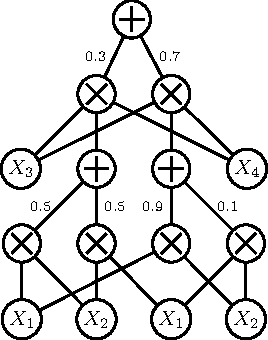
\includegraphics[width=0.7\linewidth]{figures/spn}\\
        % \begin{minipage}[t]{0.48\linewidth}
        %   \scriptsize \flushleft
        %   \textcolor{tractable_green}{\cmark \textbf{EVI}},
        %   \textcolor{tractable_green}{\cmark \textbf{SAM}},
        %   \textcolor{tractable_green}{\cmark \textbf{MAR}},\par
        %   \textcolor{tractable_green}{\cmark \textbf{CON}},
        %   \textcolor{untractable_red}{\xmark \textbf{MPE}},
        %   \textcolor{tractable_green}{\cmark \textbf{Z}}
        % \end{minipage}
        \textbf{\emph{\textcolor{tractable_green}{Computational Graphs}}}\\[20pt]
      \end{center}
    \end{minipage}\hfill\begin{minipage}[t]{0.29\linewidth}
      \begin{center}
        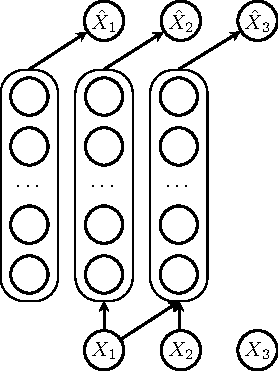
\includegraphics[width=0.8\linewidth]{figures/nade}\\
        % \begin{minipage}[t]{0.57\linewidth}
        %   \scriptsize \flushleft
        %   \textcolor{tractable_green}{\cmark \textbf{EVI}},
        %   \textcolor{tractable_green}{\cmark \textbf{SAM}},
        %   \textcolor{untractable_red}{\xmark \textbf{MAR}},\par
        %   \textcolor{untractable_red}{\xmark \textbf{CON}},
        %   \textcolor{untractable_red}{\xmark \textbf{MPE}},
        %   \textcolor{untractable_red}{\xmark \textbf{Z}}
        % \end{minipage}
        \textbf{\emph{\textcolor{tractable_green}{Autoregressive NNs}}}\\[20pt]
      \end{center}
    \end{minipage}
  \end{center}\vspace{7pt}
  $\rightarrow$ TPMs allow \textbf{exact} inference to be computed in \textbf{\textcolor{tractable_green}{polynomial time}}!
\end{frame}


\begin{frame}[t]
  \small
  \frametitle{Representation learning with TPMs}
  
  Given a set of i.i.d samples $\{\mathbf x^i\}_{i=1}^m\sim
  \mathbf{X}$,  a TPM $\theta$,  we want to generate an embedding
  $\mathbf{e}^{i}\in\mathbb{R}^{d}$ for
  each sample $i$ such as:
  
  $$\mathbf{e}^{i}=f_{p,\theta}(\mathbf{x}^{i})$$
  
  with $f$ being the transformation by $\theta$
  encoding the distribution $p(\mathbf{X})$.\\[10pt]
  
  \emph{Idea}: evaluate $\theta$ \emph{\textbf{several}} times by constructing \emph{\textbf{random
    queries}} (e.g. sample $\mathbf{Q}_{j} \subseteq \mathbf{X}, j =
  1\dots,d$),
  then use the probability value of each query as an embedding component:
  
  $$e_{j}^{i}=p_{\theta}(\mathbf{Q}_{j}=\mathbf{x}^{i}_{\mathbf{Q}_{j}})$$\\[10pt]

  $\rightarrow$ \underline{reuse} previously learned models, as \emph{black boxes}\par
  $\rightarrow$ \underline{exploit} embeddings for clustering, classification,\dots
  
  
\end{frame}

\begin{frame}[t]
  \frametitle{Experimental evaluation}
  \small
  \begin{enumerate}[I]
  \item Learning \textsf{SPNs} and \textsf{MTs} unsupervisedly on five
    binary image datasets
  \item extract embeddings from 1000 random marginal queries
  \item train a supervised linear classifier on them 
  \end{enumerate}
  \hspace{15pt}$\rightarrow$ \emph{\textbf{meaningful representations} if better accuracy scores}\\[7pt]
  \begin{center}
     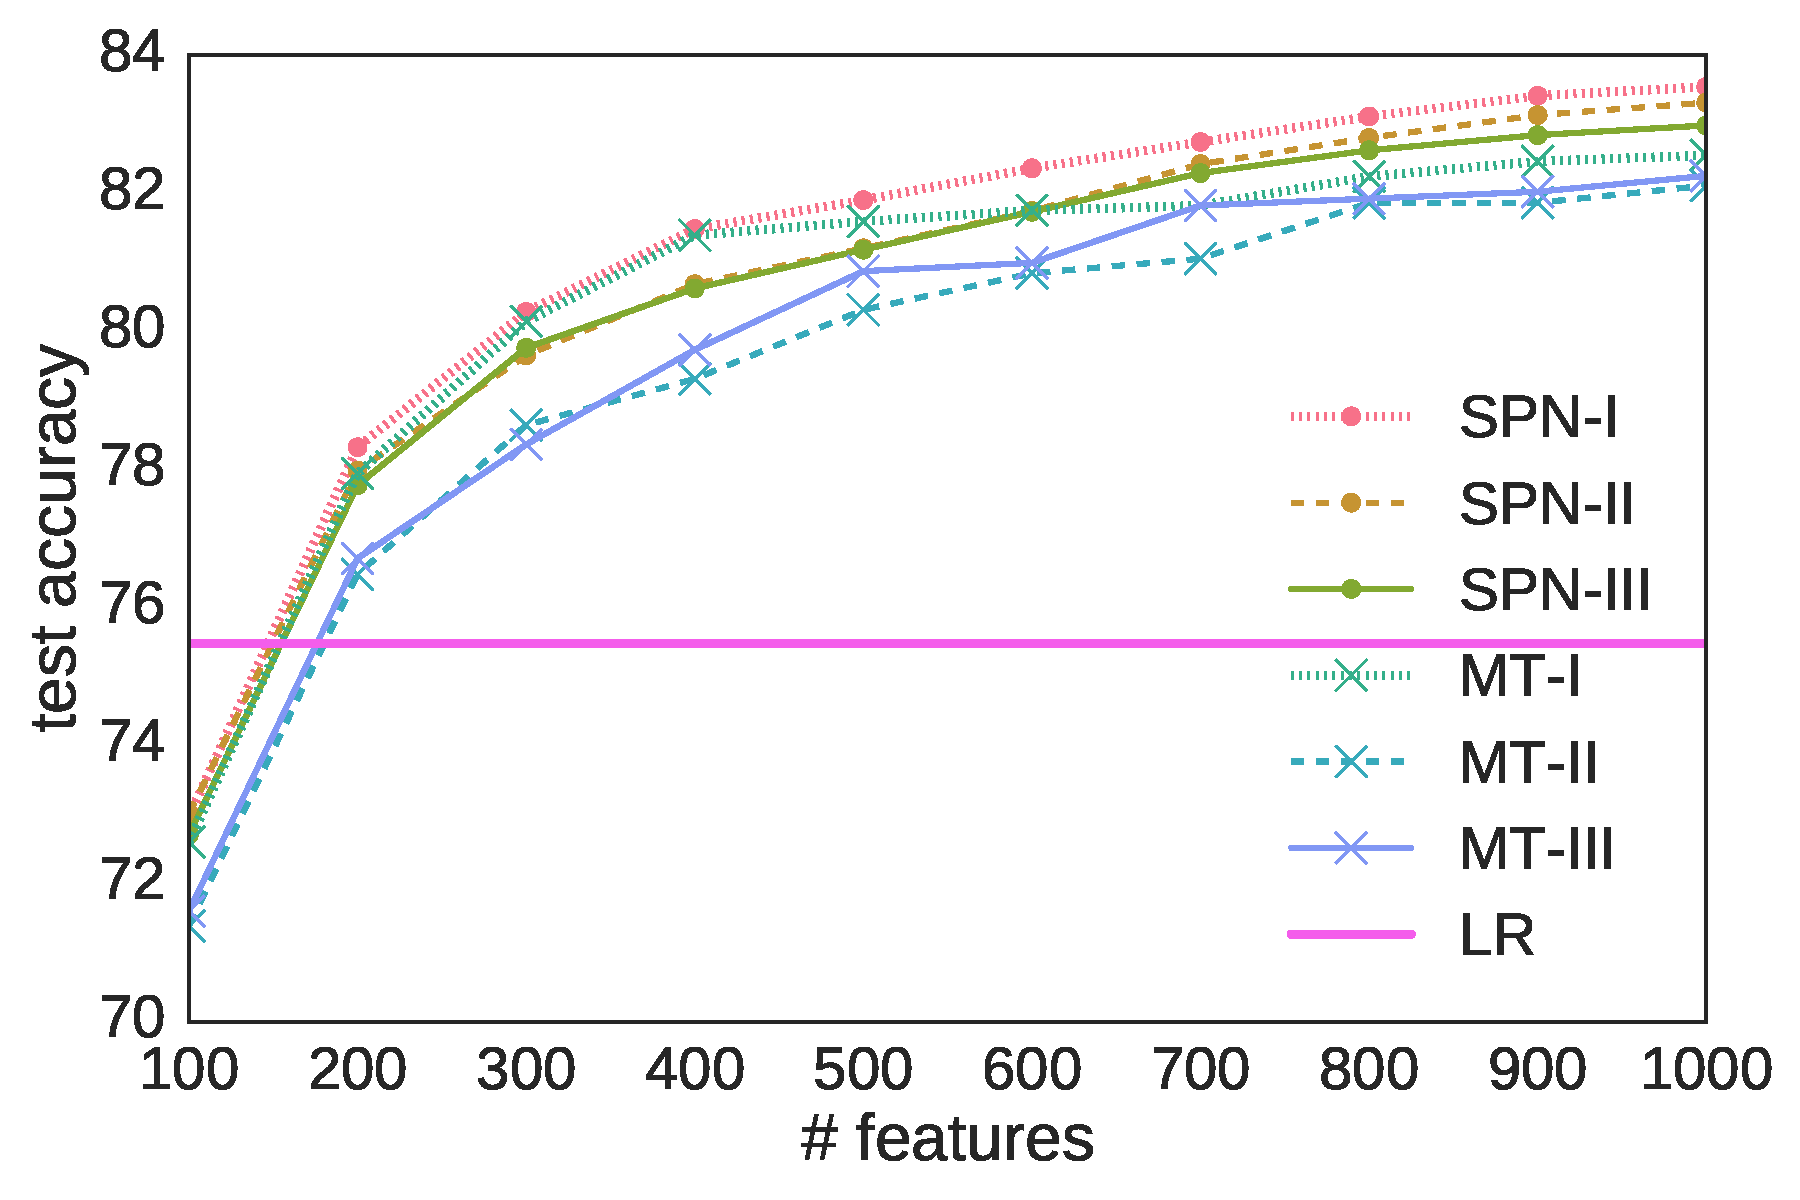
\includegraphics[width=0.47\linewidth]{figures/lines-ocr_letters}\hfill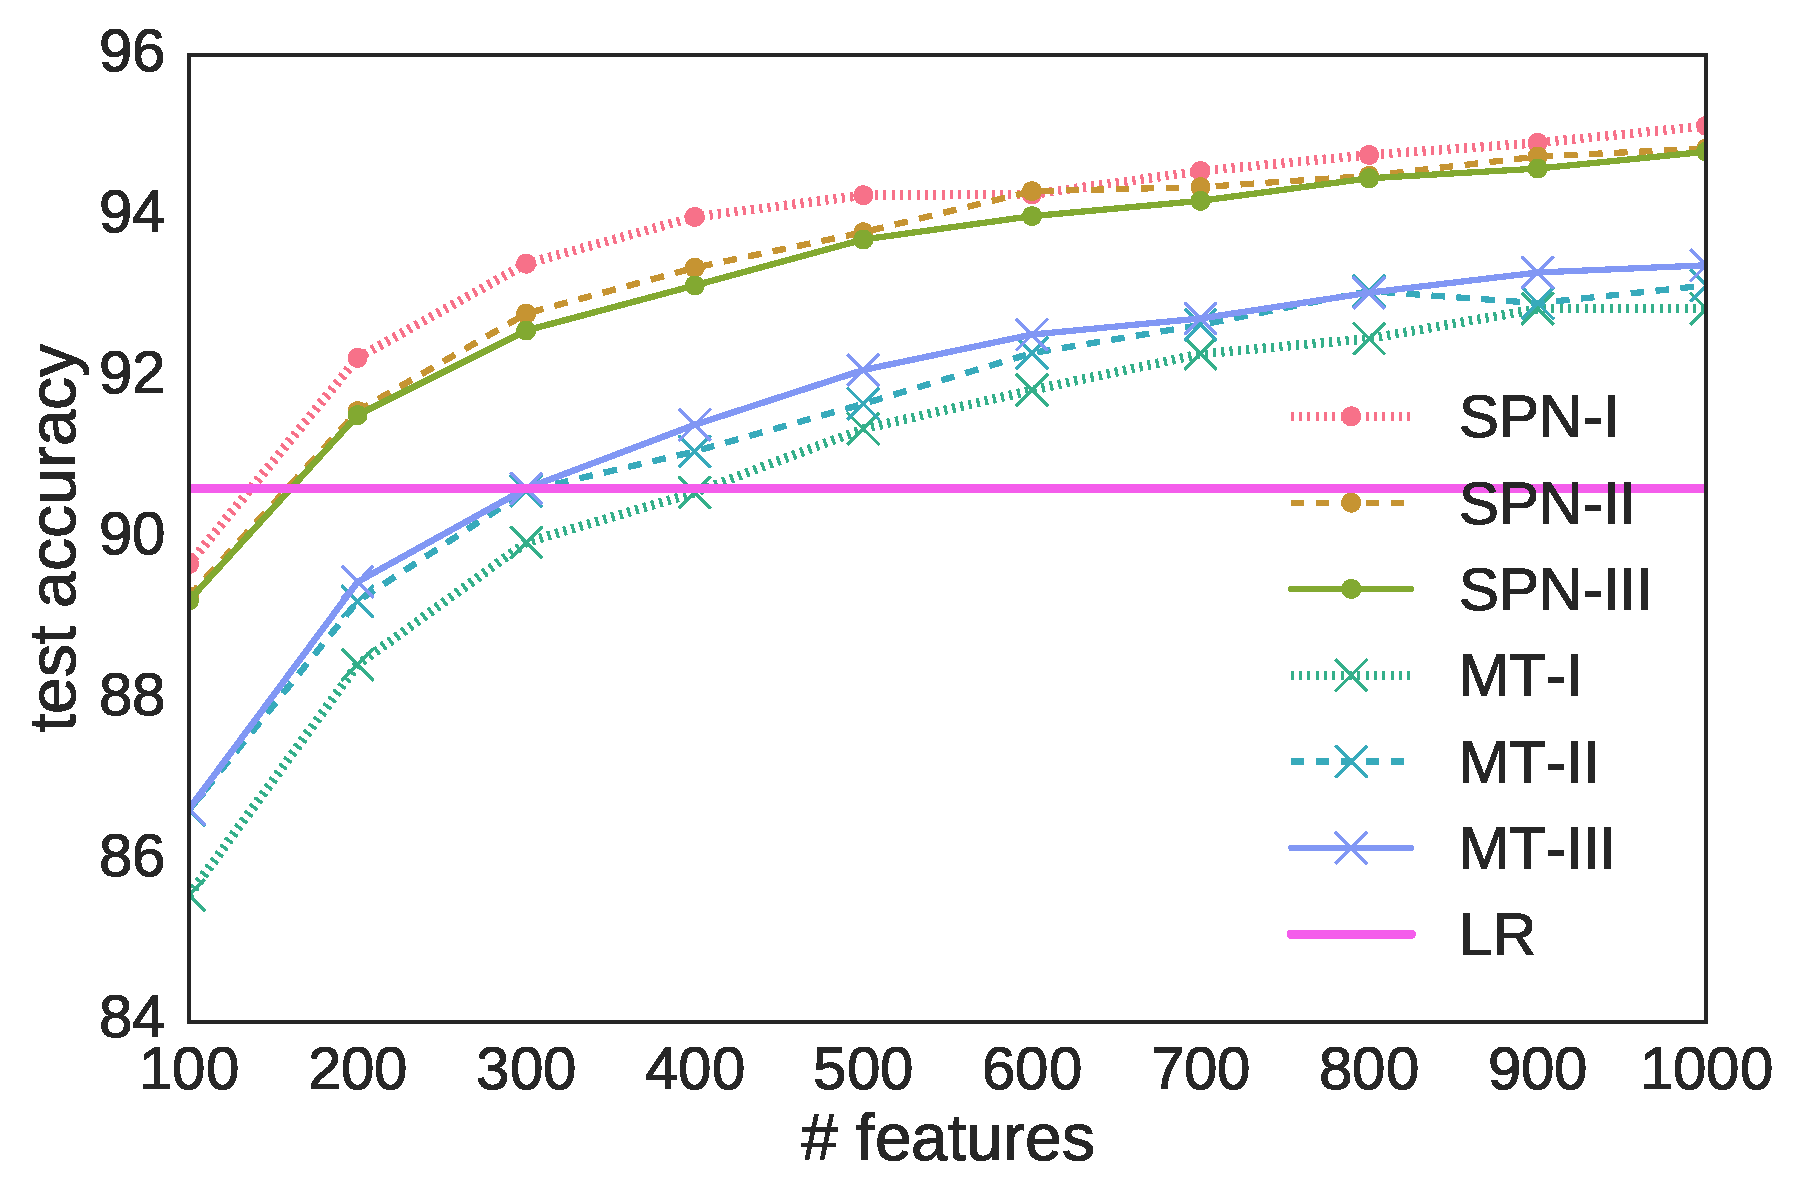
\includegraphics[width=0.47\linewidth]{figures/lines-bmnist}
   \end{center}
   \hspace{15pt}$\rightarrow$ \underline{trade-off} between likelihood over $\mathbf{X}$ and
   accuracy over $Y$
\end{frame}

\end{document}

%%% Local Variables:
%%% mode: latex
%%% TeX-engine: xetex
%%% TeX-master: t
%%% End:
